\documentclass[a4paper,12pt]{article}
\usepackage{color}
\usepackage{graphicx}
\usepackage{hyperref}
\begin{document}

\title{Dokumentation}
\author{Radike, Sauer, Wolf}
\date{\today}
\maketitle
\tableofcontents
\section{Einleitung}
This is the introduction.

\section{Entwicklung}
\subsection{erste Schrittte}
\subsubsection{Verwendung der VGA Schnittstelle}
\subsubsection{Verwendung der ADCs}
Das DE10-Lite Board hat 6 integrierte ADCs. Diese sind mit einer Bandbreite von 12 Bit und einer Sampling-Frequenz von 10 MHz spezifiziert und haben eine Verstärkerschaltung vorgeschalten. Eine analoge Eingangsspannung von 0-5V ist zulässig. Quartus-Prime bietet bereits fertige IP-Cores zur erleichterten Implementierung an.
 
\paragraph{ADC Hardware}
Die auf dem Chip \textit{MAX 10 10M50DAF484C7G} realisierten 6 ADCs werden verwendet, so ist kein extra Chip für die Analog-Digital-Wandlung notwendig. Diese ADCs haben eine Auflösung von 12 Bit, eine ADC Clock-frequency von 10MHz und verwenden die interne Referenzspannung von 2,5V. Herausgeführt sind die ADC-Pins \textbf{indirekt} an den sogenannten Arduino-Pins, wie in Abbildung \ref{ADC_Blockschaltbild} zu sehen.
\begin{figure}[!h]
\begin{center}
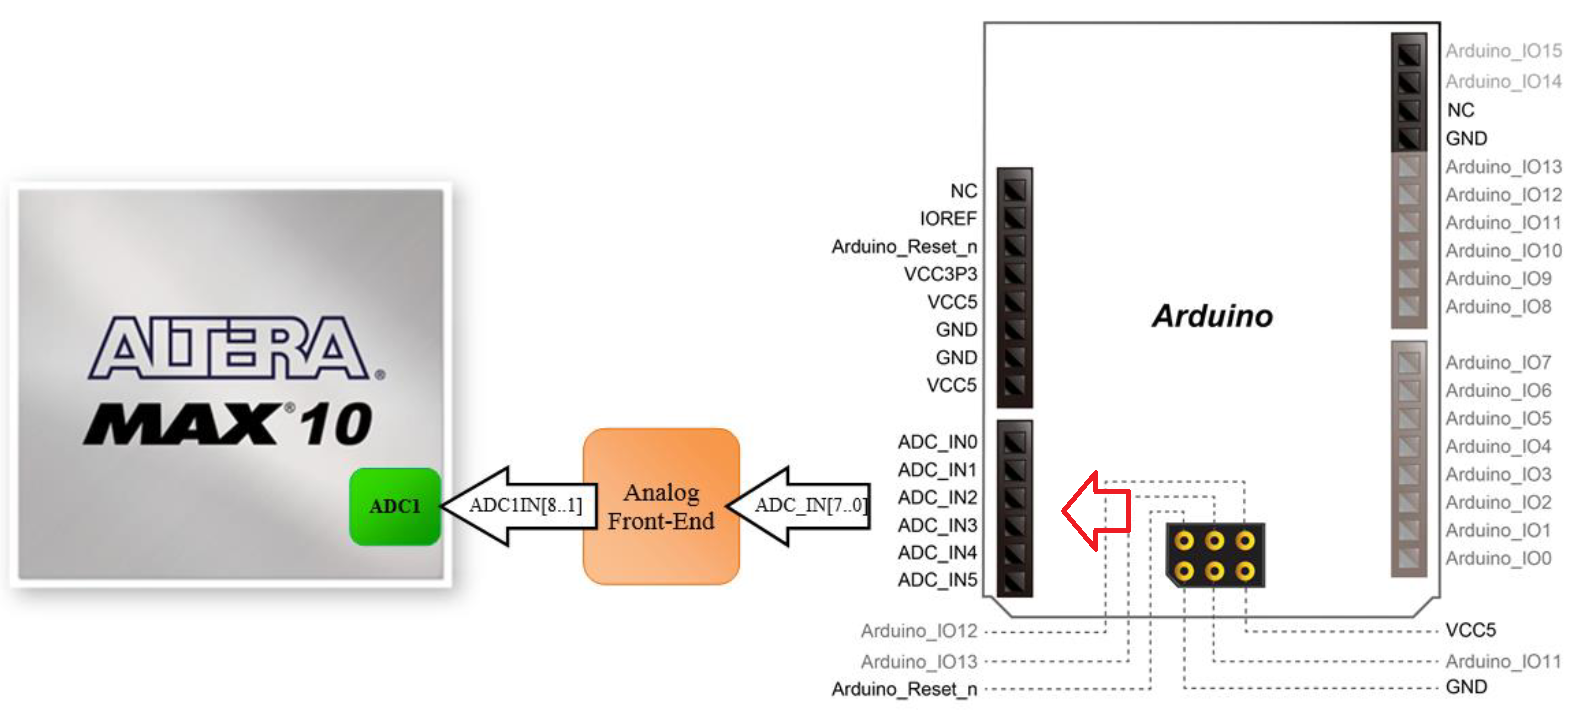
\includegraphics[width=15cm]{Grafiken/ADC_Arduino_Pins.PNG}
\caption{Blockschaltbild}
\label{ADC_Blockschaltbild}
\end{center}
\end{figure}
Das "analog Front-End" besteht aus einem OPV, der grundsätzlich die Aufgabe hat die Spannung zu halbieren. Somit werden die maximal zulässigen 5V auf 2,5V heruntergeregelt, welche die Referenzspannung des ADCs ist und diesen so auch aussteuert. Die Transitfrequenz des MCP6244 liegt bei 550kHz. Bei 10MHz geht sich eine Verstärkung von 0,5 knapp aus, was jedoch wenig Bedeutung hat, da die Frequenz Eingangssignale, aufgrund der Abtastrate, ohnehin kleiner sein muss. \\Wie in dem Schaltplanausschnitt (FPGA-Schaltplan: \ref{Schaltplan_FPGA}) in Abbildung \ref{Front-End_Schaltung} zu sehen, sind auch Kondensatoren vorhanden. Das Verhalten im Frequenzbereich wurde mithilfe von LtSpice analysiert. Da der orginale OPV im Simulationsprogramm nicht spezifiziert ist, wurde der sehr ähnliche AD8624 verwendet.
\begin{figure}[!h]
\begin{center}
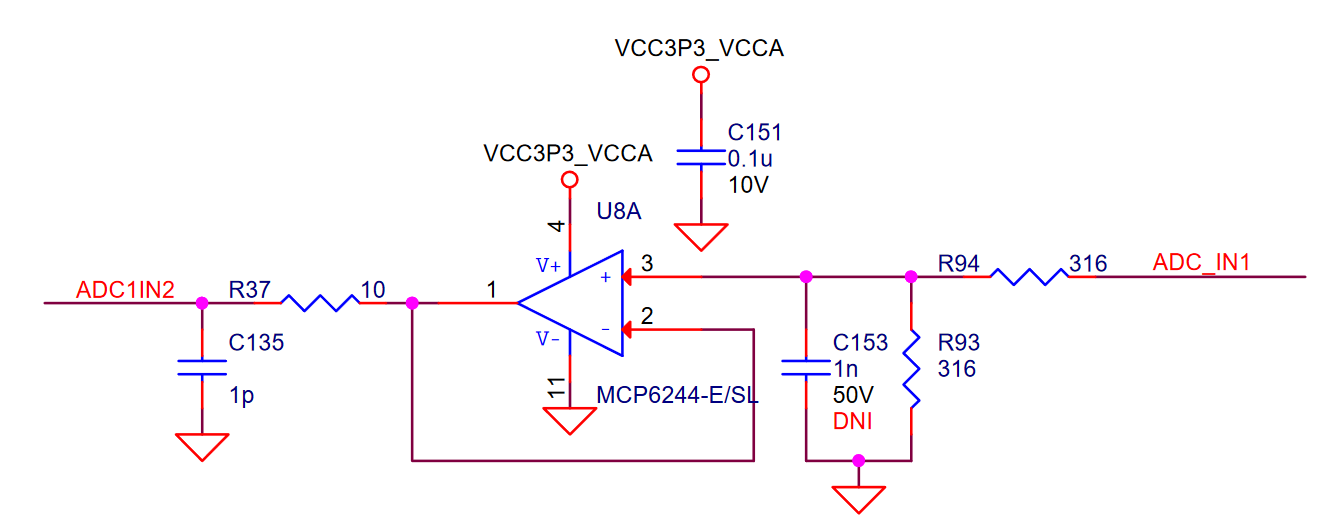
\includegraphics[width=15cm]{Grafiken/ADC_Front-End.PNG}
\caption{analog Front-End Ch1}
\label{Front-End_Schaltung}
\end{center}
\end{figure}
\newline

\paragraph{ADC VHDL-Implementierung}
a

\section{Quellen und Hilfsmittel}
\textbf{Verwendung des ADC:}
\begin{itemize}
\item Intel FPGA for Quartus Prime 17.1: Using\_DE\_Series\_ADC.pdf
\end{itemize}
\textbf{Verwendung des DE10-Lite-Boards VHDL-Programmierung:}
\begin{itemize}
\item
Übersicht: DE10-Lite-Board: DE10-Lite\_v.2.1.0\_SystemCD: DE10-Lite\_User\_Manual.pdf
\item
\label{Schaltplan_FPGA}
Schaltplan: DE10-Lite-Board: DE10-Lite\_v.2.1.0\_SystemCD: de10-lite.pdf
\item
VHDL-Spezifikation: \url{https://www.nandland.com}
\end{itemize}

\end{document}